\begin{center}\small
\begin{tabularx}{\linewidth}{@{}l>{\raggedleft\arraybackslash}X>{\raggedleft\arraybackslash}X>{\raggedleft\arraybackslash}X>{\raggedleft\arraybackslash}X@{}}
\toprule
Parameter & IID SD & HAC(30) SD & GLS SD & Full-curvature SD\\
\midrule
$K$ & 0.0008118 & 0.003714 & 0.005981 & 0.00598\\
$\tau$ & 0.1453 & 0.6578 & 1.235 & 1.232\\
$\theta$ & 0.04781 & 0.2226 & 0.288 & 0.286\\
\bottomrule
\end{tabularx}
\end{center}
SD units are $\C/\%$ for $K$ and seconds for the time constants. HAC changes the estimated OLS covariance while retaining its mean fit. IID and GLS use their own fitted means; their comparison includes the change in fitting criterion. GLS holds the covariance fixed. Full curvature includes noise estimation but remains a local, single-basin diagnostic.
\begin{center}\small
\begin{tabularx}{\linewidth}{@{}l>{\raggedleft\arraybackslash}X>{\raggedleft\arraybackslash}X@{}}
\toprule
Parameter & Gaussian 95\% range & Block 95\% range\\
\midrule
$K$ & [0.737, 0.757] & [0.737, 0.753]\\
$\tau$ & [145.900, 150.008] & [145.756, 150.088]\\
$\theta$ & [16.093, 17.266] & [15.947, 17.202]\\
\bottomrule
\end{tabularx}
\end{center}
Bootstrap refits include noise and ambient estimation, boundaries and pole alternatives. Percentile ranges summarize the working refit distributions; coverage has not been established.
The opposite pole labeling occurs in 8/400 Gaussian and 3/400 block refits. A central interval can miss that secondary basin. The step ambient bound is active in 162/400 Gaussian refits.
Nominal profile support is $K$: [0.7361, 0.7533]; $\tau$: [145.7, 150.2]; $\theta$: [16.02, 17.14]. Finite grid and crossing brackets are retained in the numerical archive.
\begin{figure}[htbp]\centering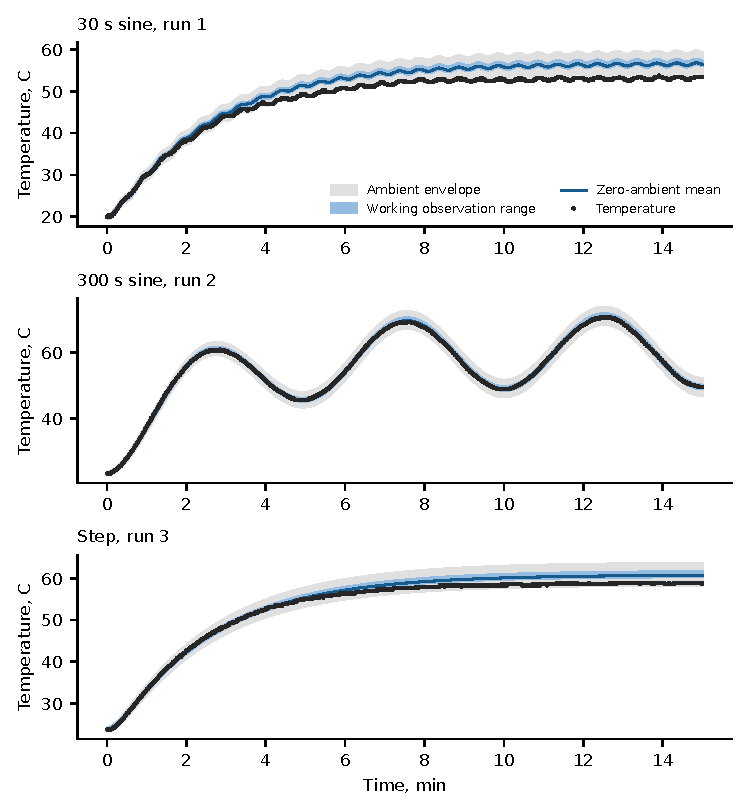
\includegraphics[width=\linewidth]{generated_release/figures/P1_predictions.pdf}\caption{P1 predictions for three evaluation records. Blue bands are pointwise Gaussian working observation ranges at zero future ambient correction; gray envelopes also allow ambient offsets in $\pm2\C$. Ambient envelopes have no assigned probability. Black points are recorded temperatures.}\end{figure}
